\chapter{Il Progetto Learning Analytics Dashboard}

\section{Introduzione}

In questo capitolo verrà presentato un esempio di applicazione delle tecniche di Learning Analytics.

Il progetto, sviluppato nel corso dello stage universitario, prevede la creazione di una dashboard che visualizzi i dati presi dall'insegnamento di Probabilità e Statistica. \\
Questo corso è stato erogato dall'università Bicocca nell' anno scolastico 2017-2018 per gli studenti del corso di laurea triennale in informatica.

Per ognuno degli otto capitoli, gli studenti hanno a disposizione:

\begin{itemize}

\item Appunti delle lezioni.
\item Videolezioni.
\item Quiz di teoria e di esercizi, con alcune eccezioni:
\begin{itemize}
   \item I capitoli 1 e 4 hanno solo quello di teoria.
   \item Il capitolo 8 ha solo quello di esercizi.
\end{itemize}
\item Forum per porre domande al docente.

\end{itemize}

Inoltre, per prepararsi all'esame, sono presenti quiz di simulazione.

\clearpage

Utilizzando questo strumento il docente può rispondere alle seguenti domande:

\begin{itemize}

\item Quando studiano gli allievi? 
\item In quale mese, settimana, giorno ed ora sono più attivi?
\item Lavorano di più durante la settimana o nel week-end?
\item Di giorno o di notte?

\end{itemize}

\begin{itemize}

\item Quali sono i quiz più svolti? 
\item Quali quelli più completati dagli studenti?
\item Sono state eseguite più attività della prima parte o della seconda parte del corso?
\item Più quiz di teoria o di esercizi?
\item Qual è stato l'andamento nel corso del tempo di un determinato quiz?
   
\end{itemize}

\begin{itemize}

   \item Come è possibile dividere gli studenti in gruppi, in base al loro completamento del corso? 
   \item Quale è il gruppo più numeroso?
    
\end{itemize}

\begin{itemize}

\item Come sono andati gli esami?
\item Conviene fare i due parziali oppure il totale?
\item Le valutazioni ottenute sono in linea con quelle prese nelle simulazioni?
\item Per ogni prova, quanti studenti sono riusciti ad accedere alla seconda parte e quanti sono rimasti bloccati alla prima?
\item L'utilizzo del corso di quanto ha influenzato il voto finale?

\end{itemize}

Inoltre, lo studente può:

\begin{itemize}

\item Vedere i quiz che ha completato.
\item Confrontare il suo modo di studiare con quello degli altri.

\end{itemize}

\clearpage

\section{Creazione}

Il progetto è stato sviluppato in cinque fasi:

\begin{enumerate}

\item Analisi della letteratura e dei software commerciali.
\item Studio delle funzionalità previste.
\item Preparazione dei dati.
\item Creazione del database.
\item Creazione del sito:
\begin{enumerate}[label=\arabic*.]
\item Client. 
\item Server. 
\end{enumerate} 

\end{enumerate}

\subsection{Analisi della letteratura e dei software commerciali}

Sono stati consultati numerosi articoli e siti web riguardanti le Learning Analytics Dashboard, per comprendere cosa potessero fare e quali fossero i loro limiti.

In particole, le seguenti pubblicazioni sono state un'utilissima fonte di ispirazione:

\begin{itemize}

\item Yeonjeong Park, Il-Hyun Jo - Development of the Learning Analytics Dashboard to Support Students’ Learning Performance
\item Corrin, de Barba - Exploring students' interpretation of feedback delivered through learning analytics dashboards
\item Tinne De Laet - Learning dashboards for actionable feedback

\end{itemize}

Inoltre, si è analizzato le funzionalità di alcuni software commerciali,
tra cui Watershed \cite{Watershed} e Zoola Analytics \cite{Zoola}, oltre ai già citati Intelliboard e StREAM.

\subsection{Studio delle funzionalità previste}

Grazie al materiale consultato durante la prima fase dello sviluppo, le conoscenze tecniche, il tempo e i dati a disposizione, si è stabilito l'elenco delle funzionalità del software. \\
Ovvero, quelle indicate nella sezione introduttiva.

\subsection{Dati utilizzati}

\subsubsection{Descrizione}

Grazie a Moodle, il Learning Management System che gestisce il corso, è stato possibile estrarre i dati dagli studenti, divisi in 24 file .csv:

\begin{itemize}

\item 1: Contiene le azioni svolte dagli studenti dal 18/01/ al 22/11/2018:
\begin{itemize}
   \item 487912 Righe
   \item Ogni riga corrisponde all'azione compiuta da uno studente
   \item 7 Colonne:
   \begin{enumerate}
      \item Data/Ora
      \item Contesto
      \item Componente
      \item Evento
      \item Descrizione
      \item Origine
      \item Indirizzo IP
   \end{enumerate}
\end{itemize}

\item 2: Strutturato come il primo file, a cui si aggiunge la colonna che indica il numero di matricola dello studente che svolge l'azione.

\item 3-6: Contengono i dati relativi agli studenti che hanno eseguito le simulazioni per i parziali:
\begin{itemize}
\item 3: Simulazioni - Primo Parziale - Teoria
\item 4: Simulazioni - Primo Parziale - Esercizi
\item 5: Simulazioni - Secondo Parziale - Teoria
\item 6: Simulazioni - Secondo Parziale - Esercizi
\item Le colonne variano in base alla tipologia di quiz, queste sono le colonne comuni a tutti i tipi:
\begin{enumerate}
   \item Codice identificativo (Matricola Universitaria)
   \item Stato
   \item Iniziato
   \item Completato
   \item Tempo impiegato
   \item Valutazione   
\end{enumerate}
\item Quelli di teoria hanno ulteriori dieci colonne che riportano il punteggio ottenuto in ogni domanda
\item Quelli di esercizi hanno in più due colonne contenenti la valutazione ottenuta in ciascun esercizio
\end{itemize}

\item 7-14: Contengono i dati relativi agli studenti che hanno eseguito il primo parziale:
\begin{itemize}
   \item 7: Primo Parziale - Turno 1 - Teoria
   \item 8: Primo Parziale - Turno 1 - Esercizi
   \item 9: Primo Parziale - Turno 2 - Teoria
   \item 10: Primo Parziale - Turno 2 - Esercizi
   \item 11: Primo Parziale - Turno 3 - Teoria
   \item 12: Primo Parziale - Turno 3 - Esercizi
   \item 13: Primo Parziale - Turno 4 - Teoria
   \item 14: Primo Parziale - Turno 4 - Esercizi
   \item La struttura è identica ai file di simulazione
\end{itemize}

\item 15-20: Contengono i dati relativi agli studenti che hanno eseguito il secondo parziale:
\begin{itemize}
   \item 15: Secondo Parziale - Turno 1 - Teoria
   \item 16: Secondo Parziale - Turno 1 - Esercizi
   \item 17: Secondo Parziale - Turno 2 - Teoria
   \item 18: Secondo Parziale - Turno 2 - Esercizi
   \item 19: Secondo Parziale - Turno 3 - Teoria
   \item 20: Secondo Parziale - Turno 3 - Esercizi
   \item La struttura è identica ai file di simulazione
\end{itemize}

\item 21-22: Contengono i dati relativi agli studenti che hanno eseguito il primo appello:
\begin{itemize}
   \item 21: Primo Appello - Teoria
   \item 22: Primo Appello - Esercizi
   \item La struttura è identica ai file di simulazione
\end{itemize}

\item 23-24: Contengono i dati relativi agli studenti che hanno eseguito il secondo appello:
\begin{itemize}
   \item 23: Secondo Appello - Teoria
   \item 24: Secondo Appello - Esercizi
   \item La struttura è identica ai file di simulazione
\end{itemize}

\end{itemize} 

I dati sono stati estratti una sola volta, a corso già completato.

\subsubsection{Preparazione}

Per agevolare l'analisi, si è pensato di sistemare al meglio i dati, usando il linguaggio di programmazione R \cite{R}.

Per ogni file, si è usato il comando "unique" per eliminare gli eventuali doppioni. 

Dal secondo file, dopo una serie di operazioni, si è ottenuta una tabella che mostra la correlazione tra il codice id presente nel campo Descrizione ed il numero di matricola.
Così, è stato possibile analizzare come il modo di studiare dell'allievo abbia influito sulla sua valutazione finale.

Sul primo file sono state eseguite le seguenti operazioni:
\begin{itemize}
\item I dati sono stati filtrati, per ottenere solo le righe che riguardano l'utilizzo dei quiz.
\item I nomi dei quiz sono stati modificati. In questo modo, un quiz viene indicato con un numero che identifica il capitolo e con una lettera che identifica il suo tipo.
\begin{itemize}
\item Ad esempio, 2T rappresenta il quiz di teoria del secondo capitolo.  
\end{itemize} 
\item Si è ridotta la colonna Descrizione in modo tale che contenesse solo il codice id dello studente. Successivamente, utilizzando la tabella ottenuta dal secondo file, si è convertito questo codice nella matricola.
\item La colonna descrizione è stata rinominata in Matricola e si è impostata come colonna iniziale.
\item Sono state eliminate le colonne Componente, Origine ed Indirizzo IP.
\item La colonna Data/Ora è stata spezzata in più colonne che mostrano il mese, la settimana, il giorno e l'ora in cui si è svolta l'attività.
\end{itemize}

Per quanto riguarda i file contenenti i voti delle simulazioni, dei parziali e degli appelli, si è proceduto in questo modo:
\begin{itemize}
\item Sono state tolte le colonne Stato, Completato, Tempo impiegato.
\item Per i quiz di teoria sono state eliminate le ultime 10 colonne, ovvero quelle che riportano il punteggio ottenuto in ogni domanda.
\item Per quelli di esercizi sono state rimosse le ultime 2 colonne, ovvero  quelle contenenti la valutazione ottenuta in ciascun esercizio.
\item La colonna Iniziato, contenente la data e l'ora di inizio, è stata spezzata in più colonne che mostrano il mese, la settimana, il giorno e l'ora in cui si è svolta l'attività.
\item Gli esami divisi in più turni sono stati raggruppati in un unico file.
\end{itemize}

\subsection{Creazione del database}

Un database è, molto brevemente, un programma specializzato nella gestione dei dati. Grazie a questo software, essi possono essere inseriti, letti, modificati ed eliminati. \\ Inoltre, è anche possibile selezionarne solo una parte in base a certi criteri.

Per questo progetto, si è scelto di usare Neo4j \cite{Neo4j}, un database a grafo, nel quale le informazioni sono memorizzate tramite:
\begin{itemize}
   \item Nodi: Contengono i concetti principali.
   \item Archi: Collegano tra di loro i nodi e quindi mostrano le relazioni tra dati.
\end{itemize}

Inoltre, sia nodi che archi possono avere attributi, che rappresentano le loro proprietà.

Il database, creato a partire dai dati ottenuti nella precedente fase, ha questa struttura:

\begin{itemize}
\item Ogni studente è memorizzato in un nodo, avendo il numero di matricola come unico attributo.
\item Tutti i quiz, anche quelli di simulazioni, dei parziali e degli appelli, sono memorizzati tramite nodi aventi questi attributi:
\begin{itemize}
\item Nome
\begin{itemize}
\item Per semplicità, si è deciso di accorciare i nomi con delle sigle: \\
1T = Quiz di teoria del primo capitolo, 1PST = Primo parziale simulazione teoria, 1PT = Primo parziale teoria, 1AT = Primo appello teoria \\
e così via per gli altri quiz 
\end{itemize}
\item Tipo
\begin{itemize}
\item T se il quiz è di teoria, E se il quiz è di esercizi
\end{itemize}
\item Contesto
\begin{itemize}
\item A se il quiz è una prova di appello, P se è una prova parziale, S se è una simulazione, E altrimenti 
\end{itemize}
\end{itemize}
\item Le relazioni FaQuizNormale, FaSimulazione, FaParziale, FaTotale collegano il nodo che rappresenta lo studente con le rispettive attività svolte.
\begin{itemize}
\item Grazie agli attributi, vengono salvati il mese, la settimana, il giorno e l'ora in cui si è svolta l'attività, inoltre, se quest'ultima lo prevede, anche la valutazione ottenuta.
\end{itemize} 
\end{itemize}

\subsection{Creazione del sito}

Il progetto è un normale sito web, di conseguenza è diviso in 2 parti:
\begin{itemize}
\item Client: È la parte con cui interagisce l'utente finale, è composta da grafici, immagini, bottoni e da tutto ciò che è visibile.
\item Server: È la parte che gestisce il client, si occupa di fornire le singole pagine web ed interagire con il database. 
\end{itemize}
\subsubsection{Client}

Il client è composto da pagine web, ogni pagina ha uno scopo differente ed è stata realizzata con due linguaggi che vengono quasi sempre utilizzati in questo ambito, ovvero:
\begin{itemize}
\item HTML \cite{HTML}: Definisce gli elementi presenti nella singola pagina attraverso dei tag. \\ Ad esempio, la tag <p> rappresenta un paragrafo di testo, la tag <a> indica un link, la tag <img> crea un'immagine e così via \dots
\item CSS \cite{CSS}: Si occupa della grafica della pagina, impostando, per ogni elemento, dettagli come il colore, la posizione, la dimensione, \dots
\end{itemize}

Per rendere più interattive le pagine è stato utilizzato il linguaggio di programmazione JavaScript \cite{JS}.

Quest'ultimo è stato usato anche per la creazione dei grafici, in collaborazione con il software Google Charts \cite{GC}.

\subsubsection{Server}

Il server è stato realizzato utilizzando la famosa accoppiata Node.js \cite{Node} ed Express \cite{Express}, in questo modo, è stato possibile utilizzare ancora una volta JavaScript.

Questi software permettono di:
\begin{enumerate}
\item Gestire le richieste dell'utente. \\ Ad esempio, se vuole vedere la pagina Presentazione, il server deve fare operazioni differenti rispetto a quando si visita un'altra parte del sito.
\item Ottenere i dati necessari dal database.
\item Passare quest'ultimi alla pagina scelta dall'utente, per creare cosi i grafici. \\ Questo passaggio avviene grazie al Template Engine EJS \cite{EJS}.
\end{enumerate}

\section{Presentazione}

In questa sezione, verranno mostrate alcune immagini della dashboard creata.

\subsection{Partecipazione}

\begin{figure}[H]
	\centering
	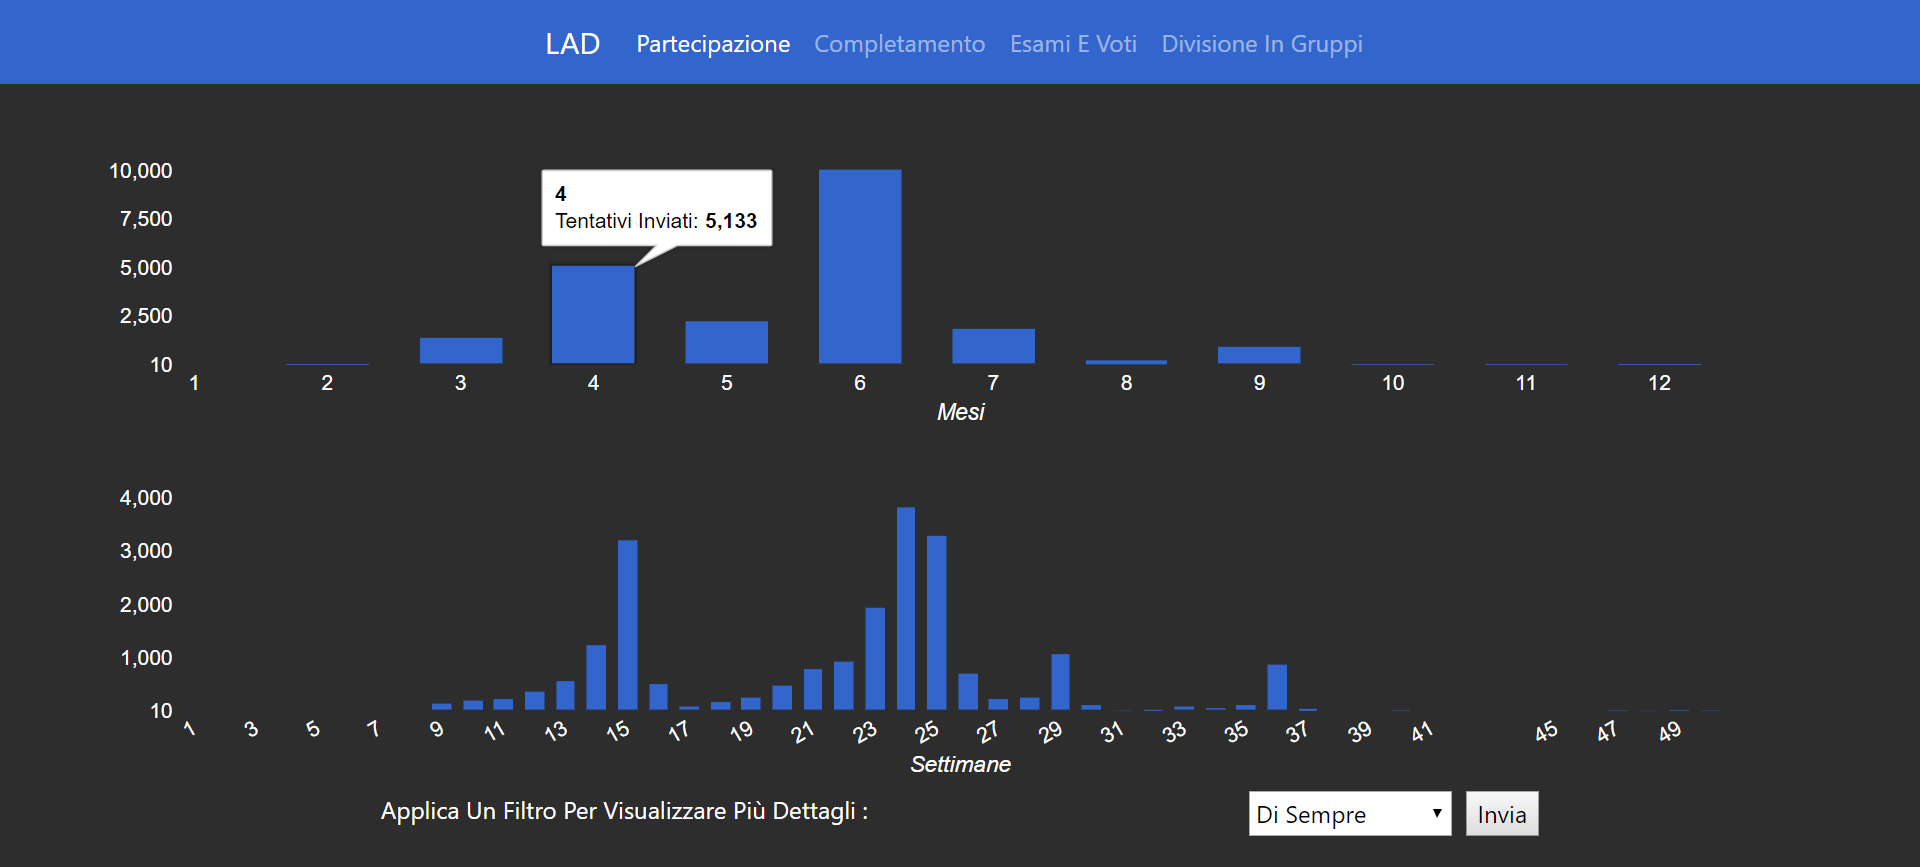
\includegraphics[width=160mm]{../Immagini/1}
\end{figure}

\begin{figure}[H]
	\centering
	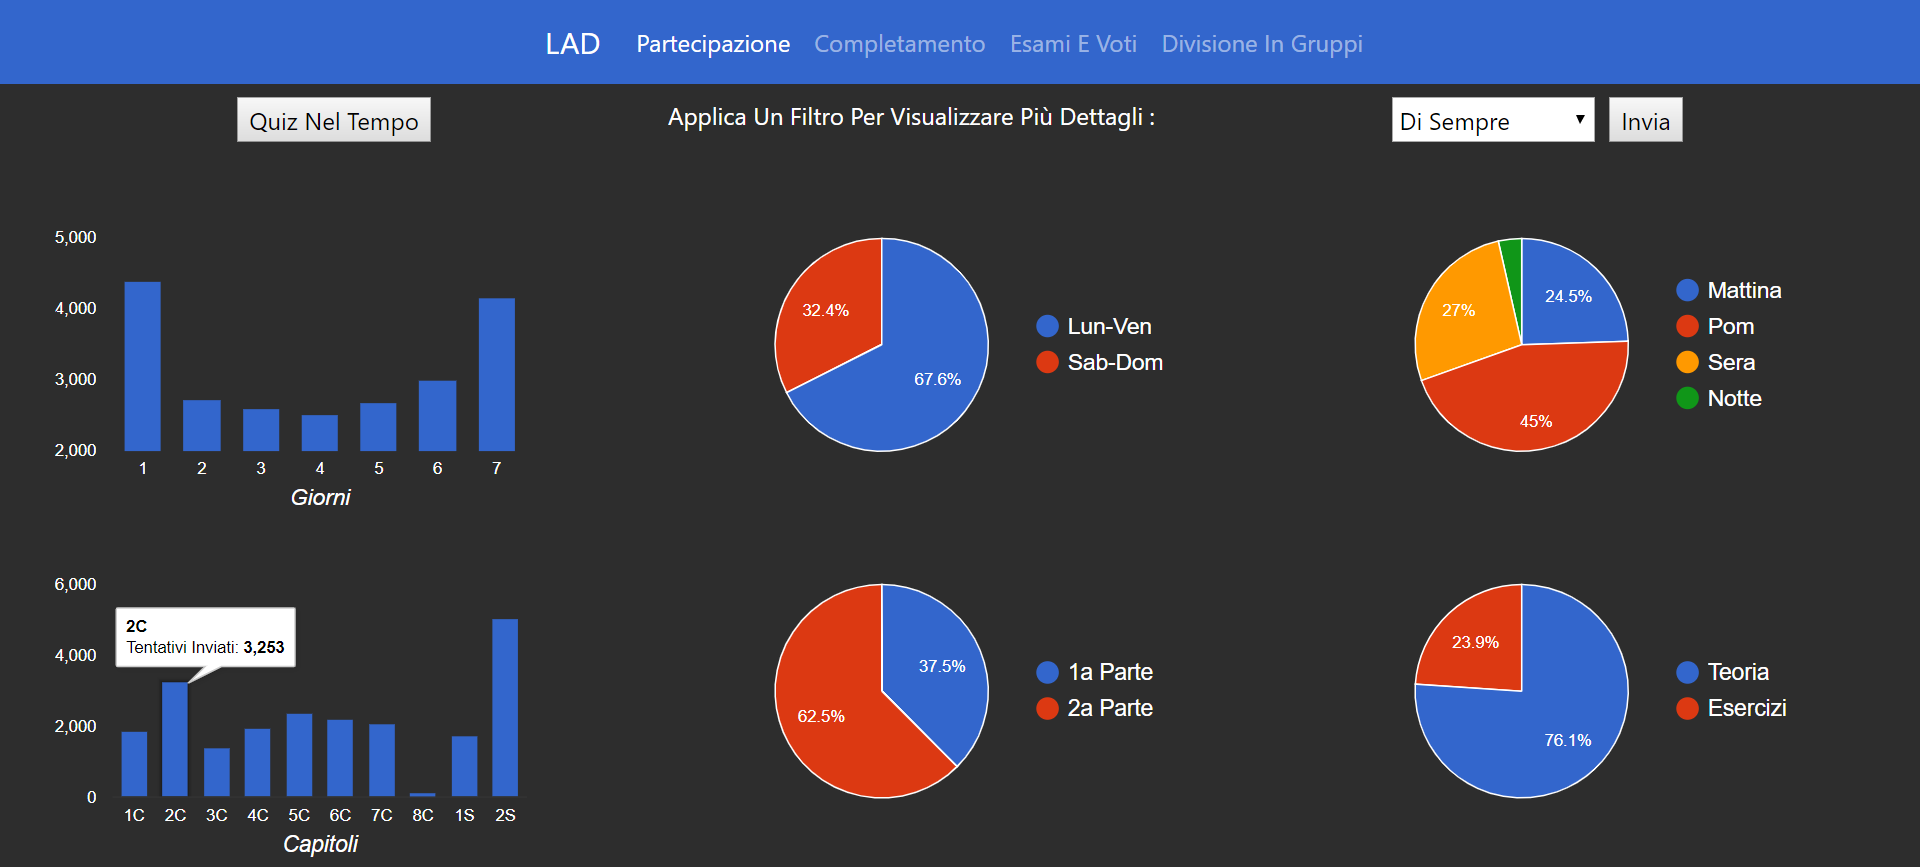
\includegraphics[width=160mm]{../Immagini/2}
\end{figure}

\begin{figure}[H]
	\centering
	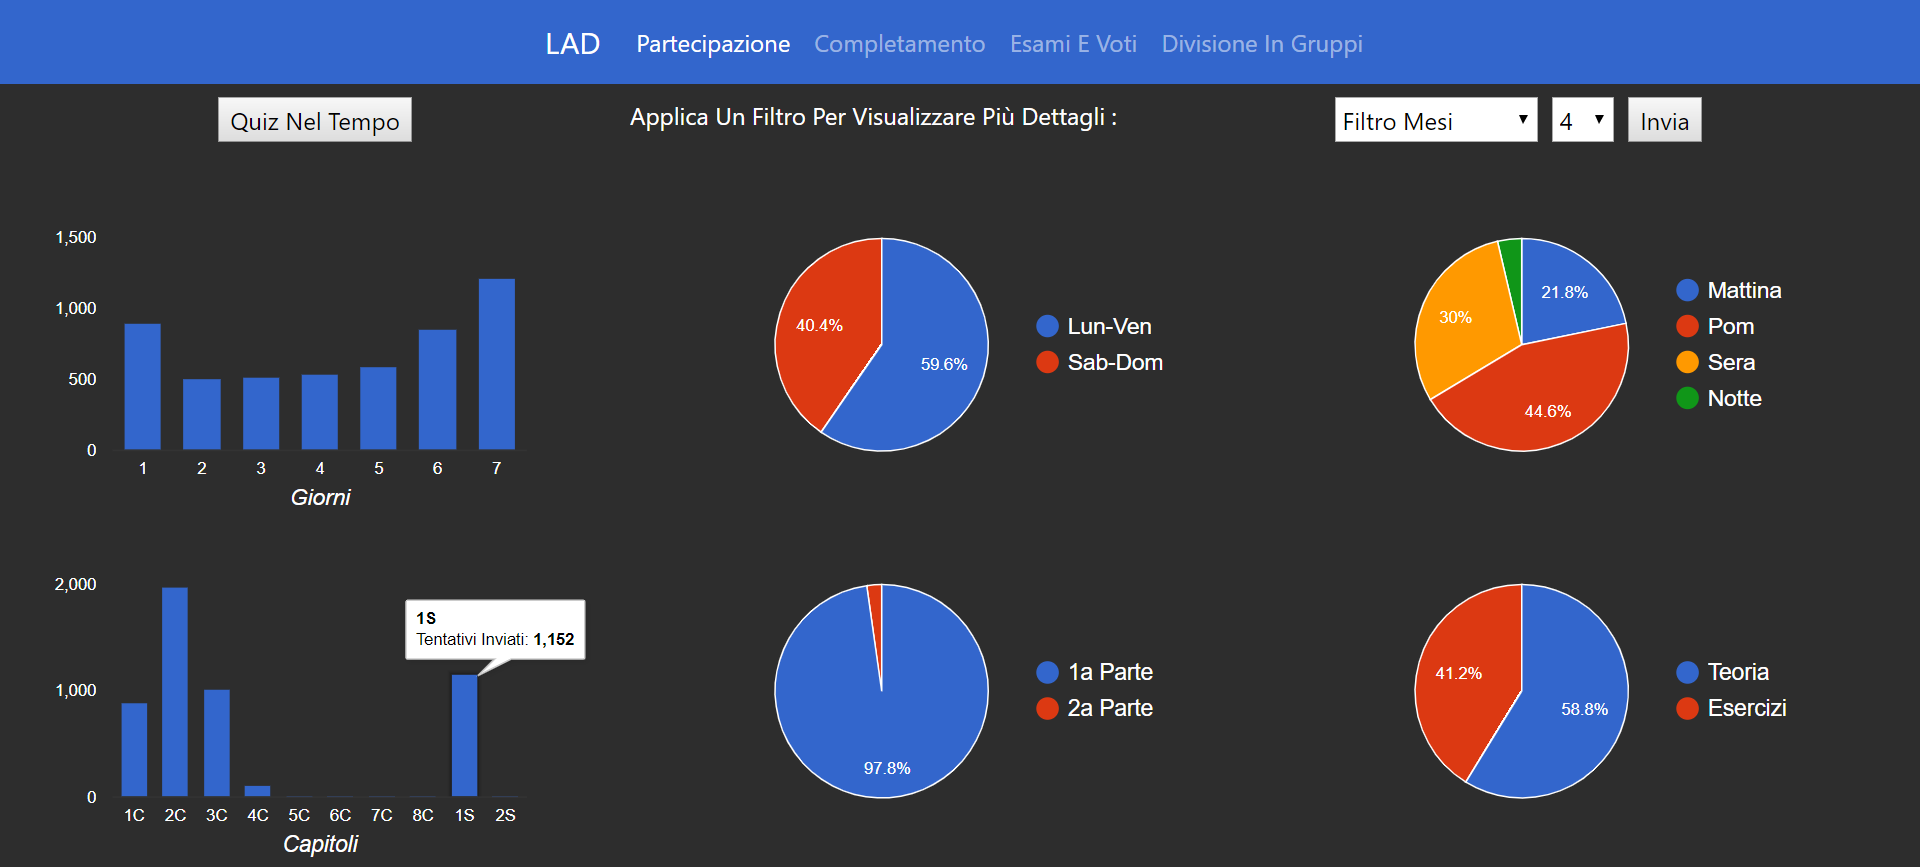
\includegraphics[width=160mm]{../Immagini/3}
\end{figure}

\begin{figure}[H]
	\centering
	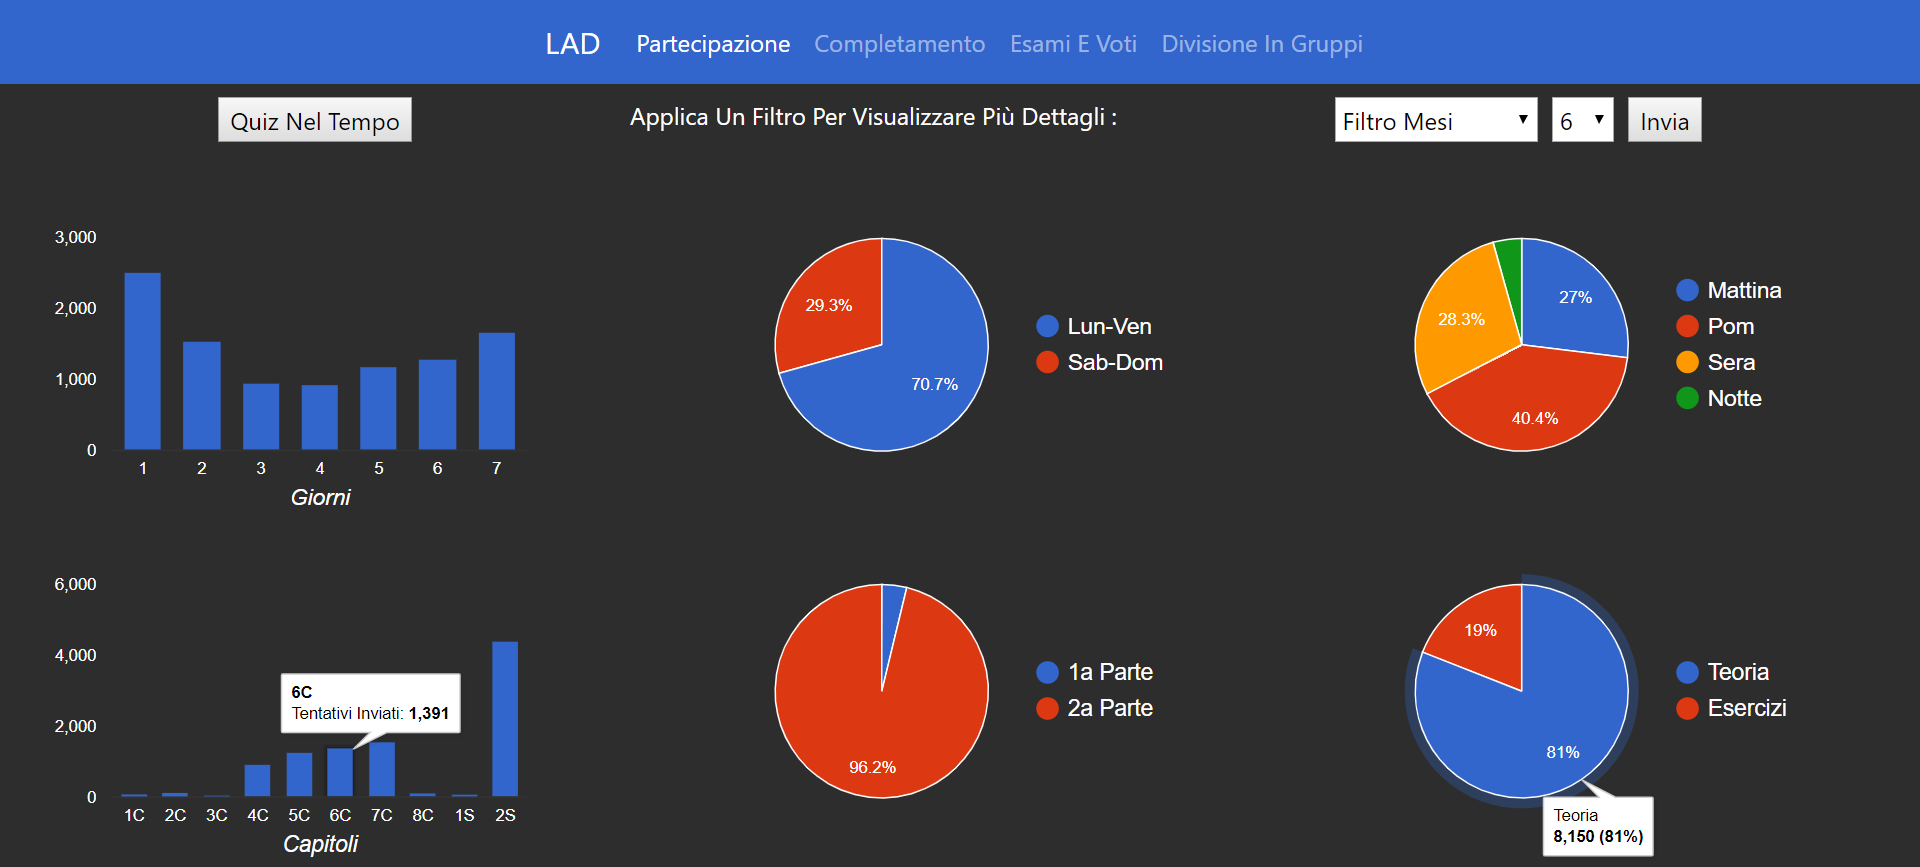
\includegraphics[width=160mm]{../Immagini/4}
\end{figure}

\begin{figure}[H]
	\centering
	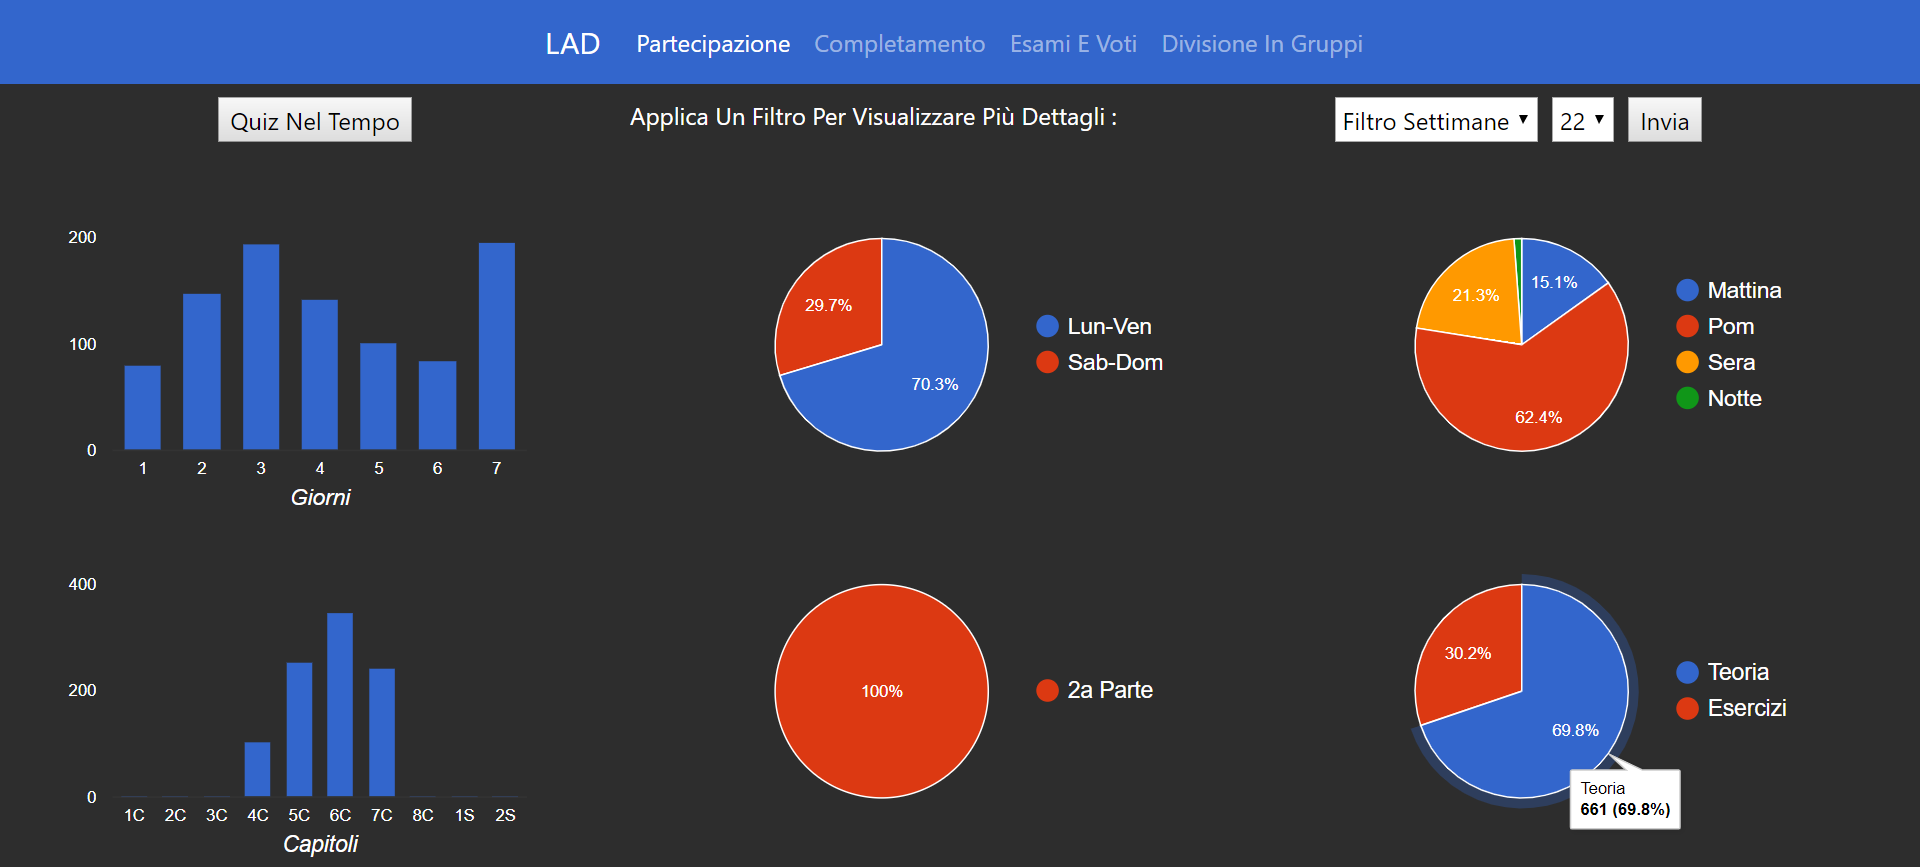
\includegraphics[width=160mm]{../Immagini/9}
\end{figure}

\subsection{Andamento Quiz}

\begin{figure}[H]
	\centering
	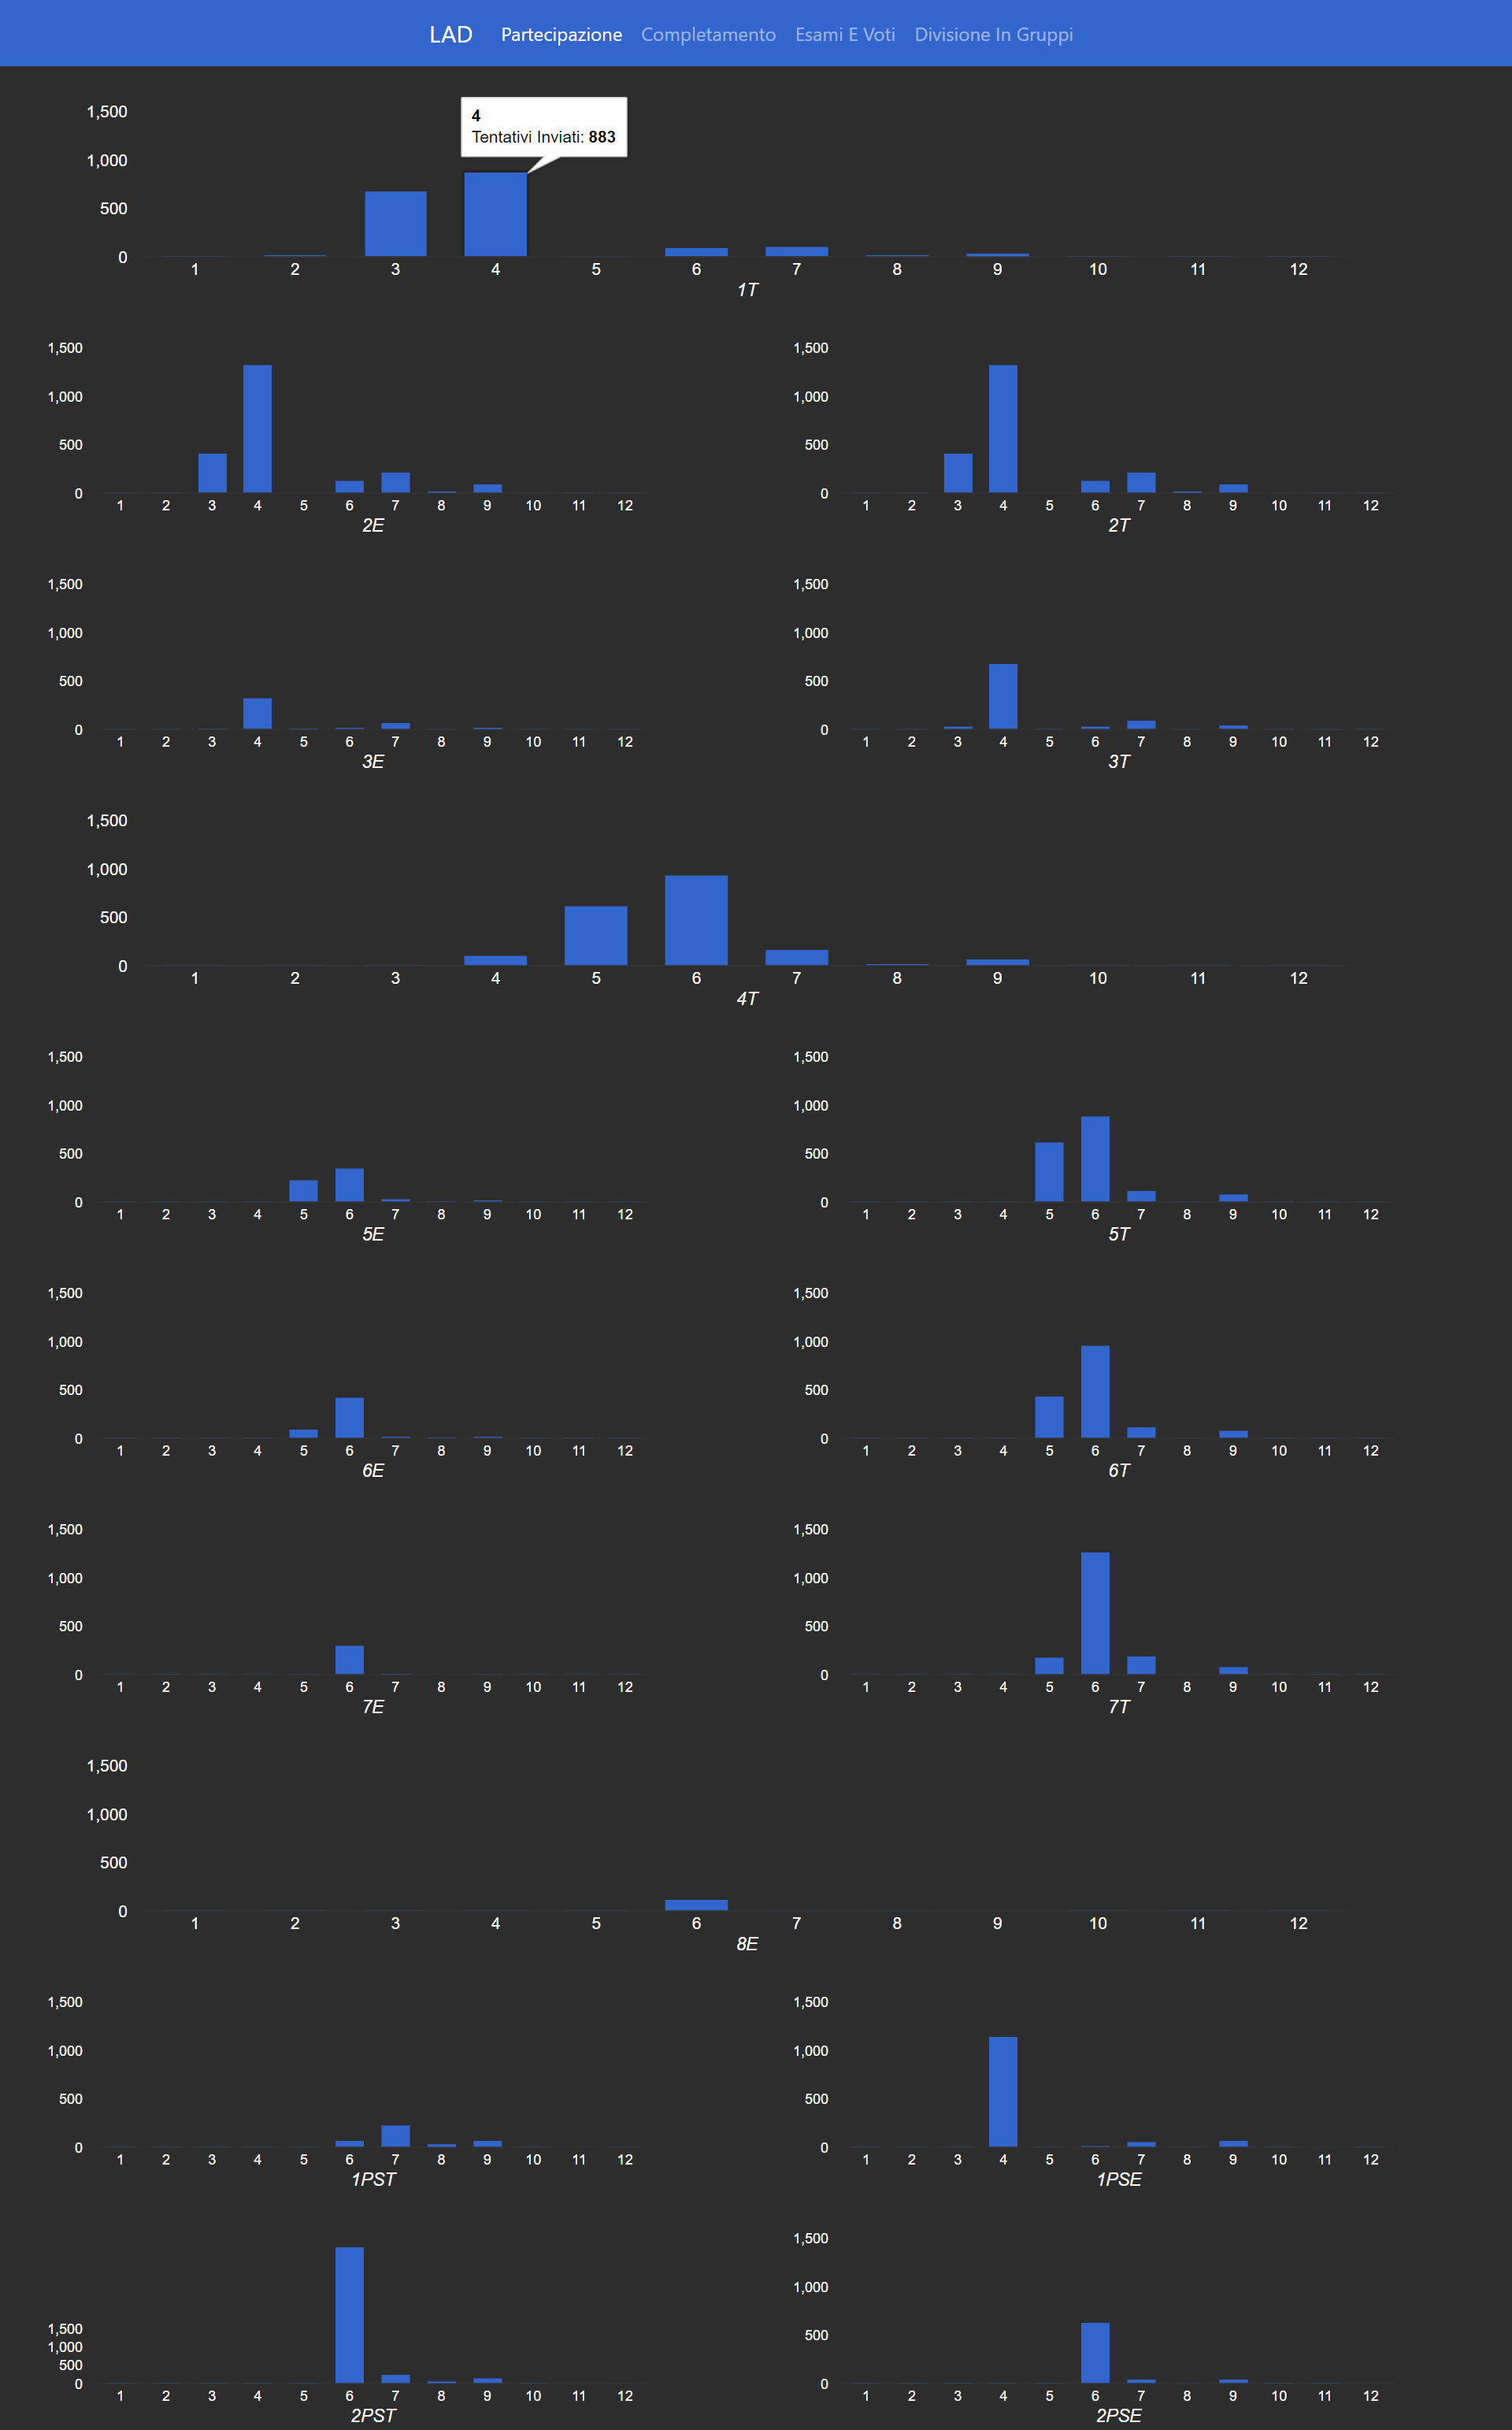
\includegraphics[width=160mm,height= 210mm]{../Immagini/5}
\end{figure}

\subsection{Completamento}

\begin{figure}[H]
	\centering
	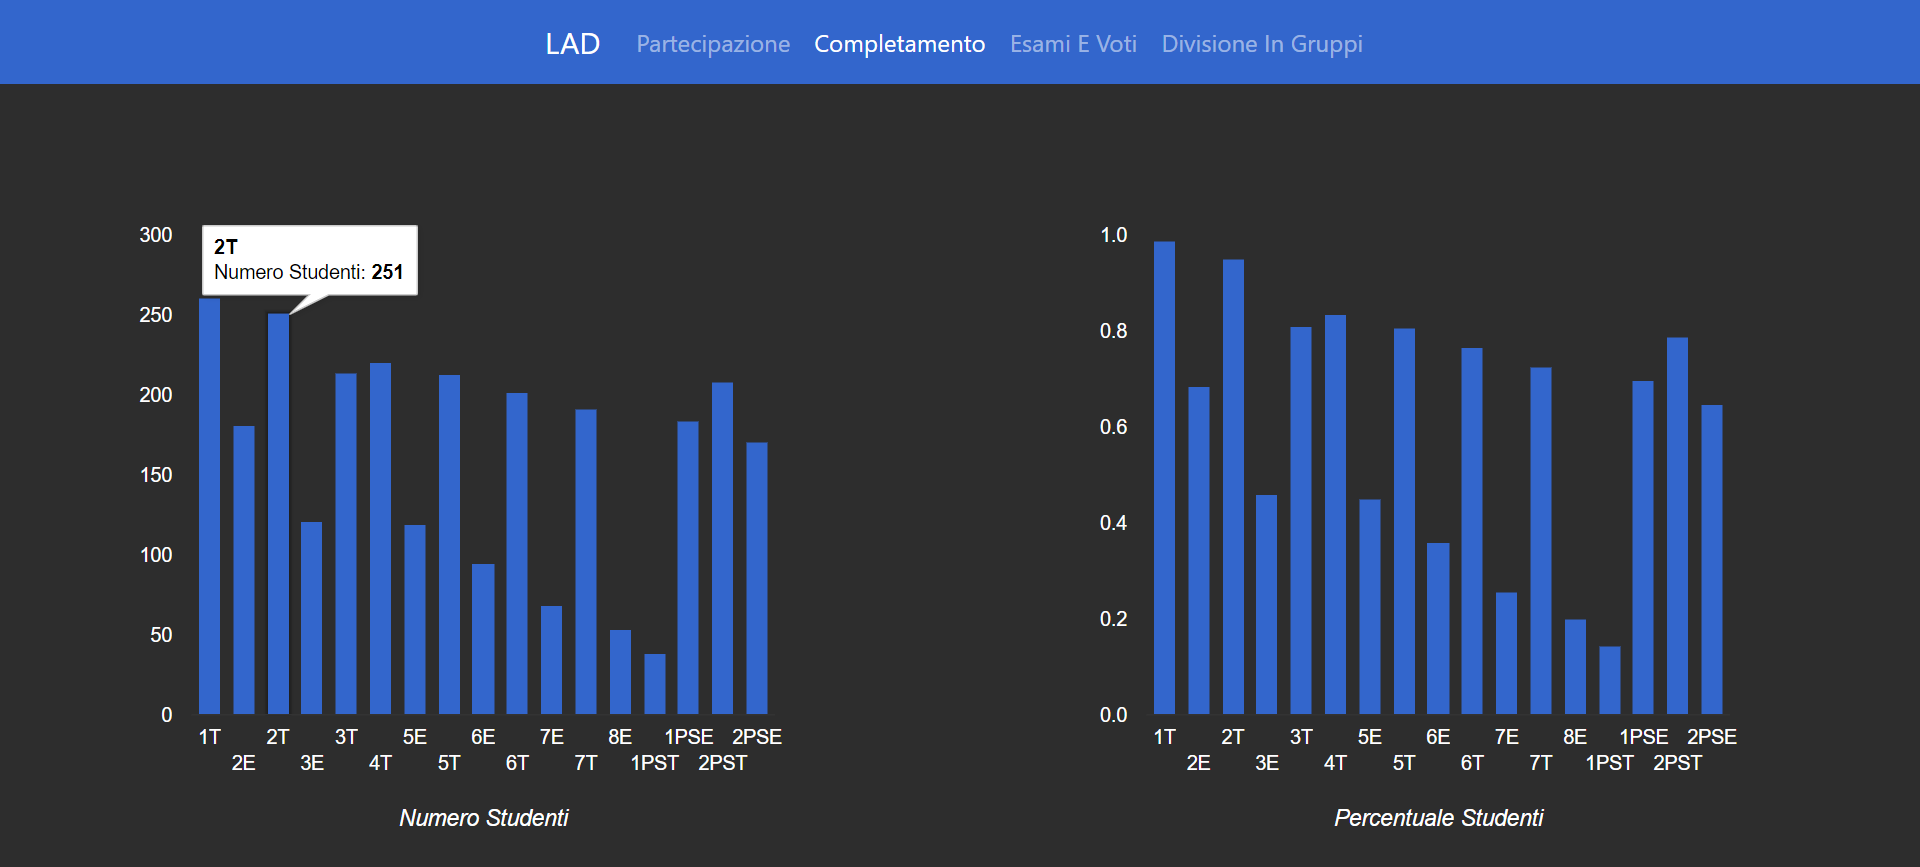
\includegraphics[width=160mm]{../Immagini/6}
\end{figure}

\subsection{Esami E Voti}

\begin{figure}[H]
	\centering
	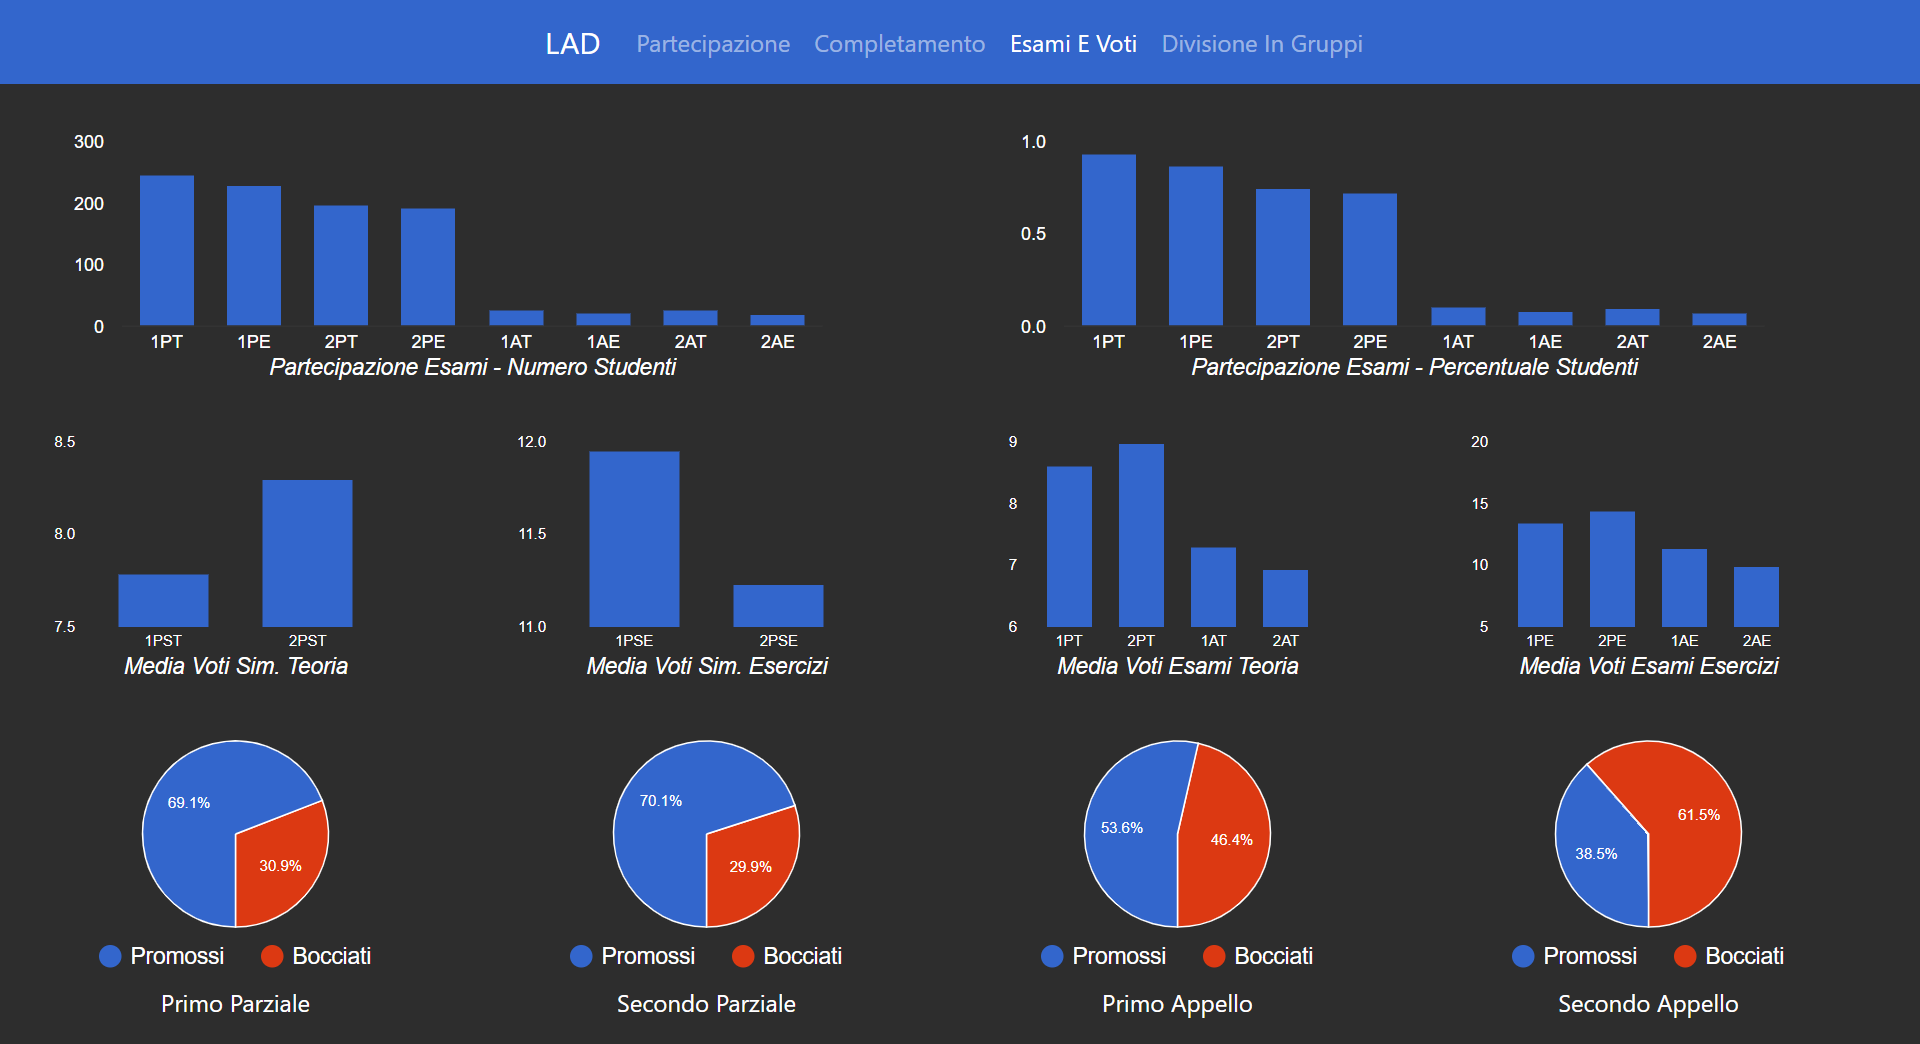
\includegraphics[width=160mm]{../Immagini/7}
\end{figure}

\subsection{Divisione In Gruppi}

\begin{figure}[H]
	\centering
	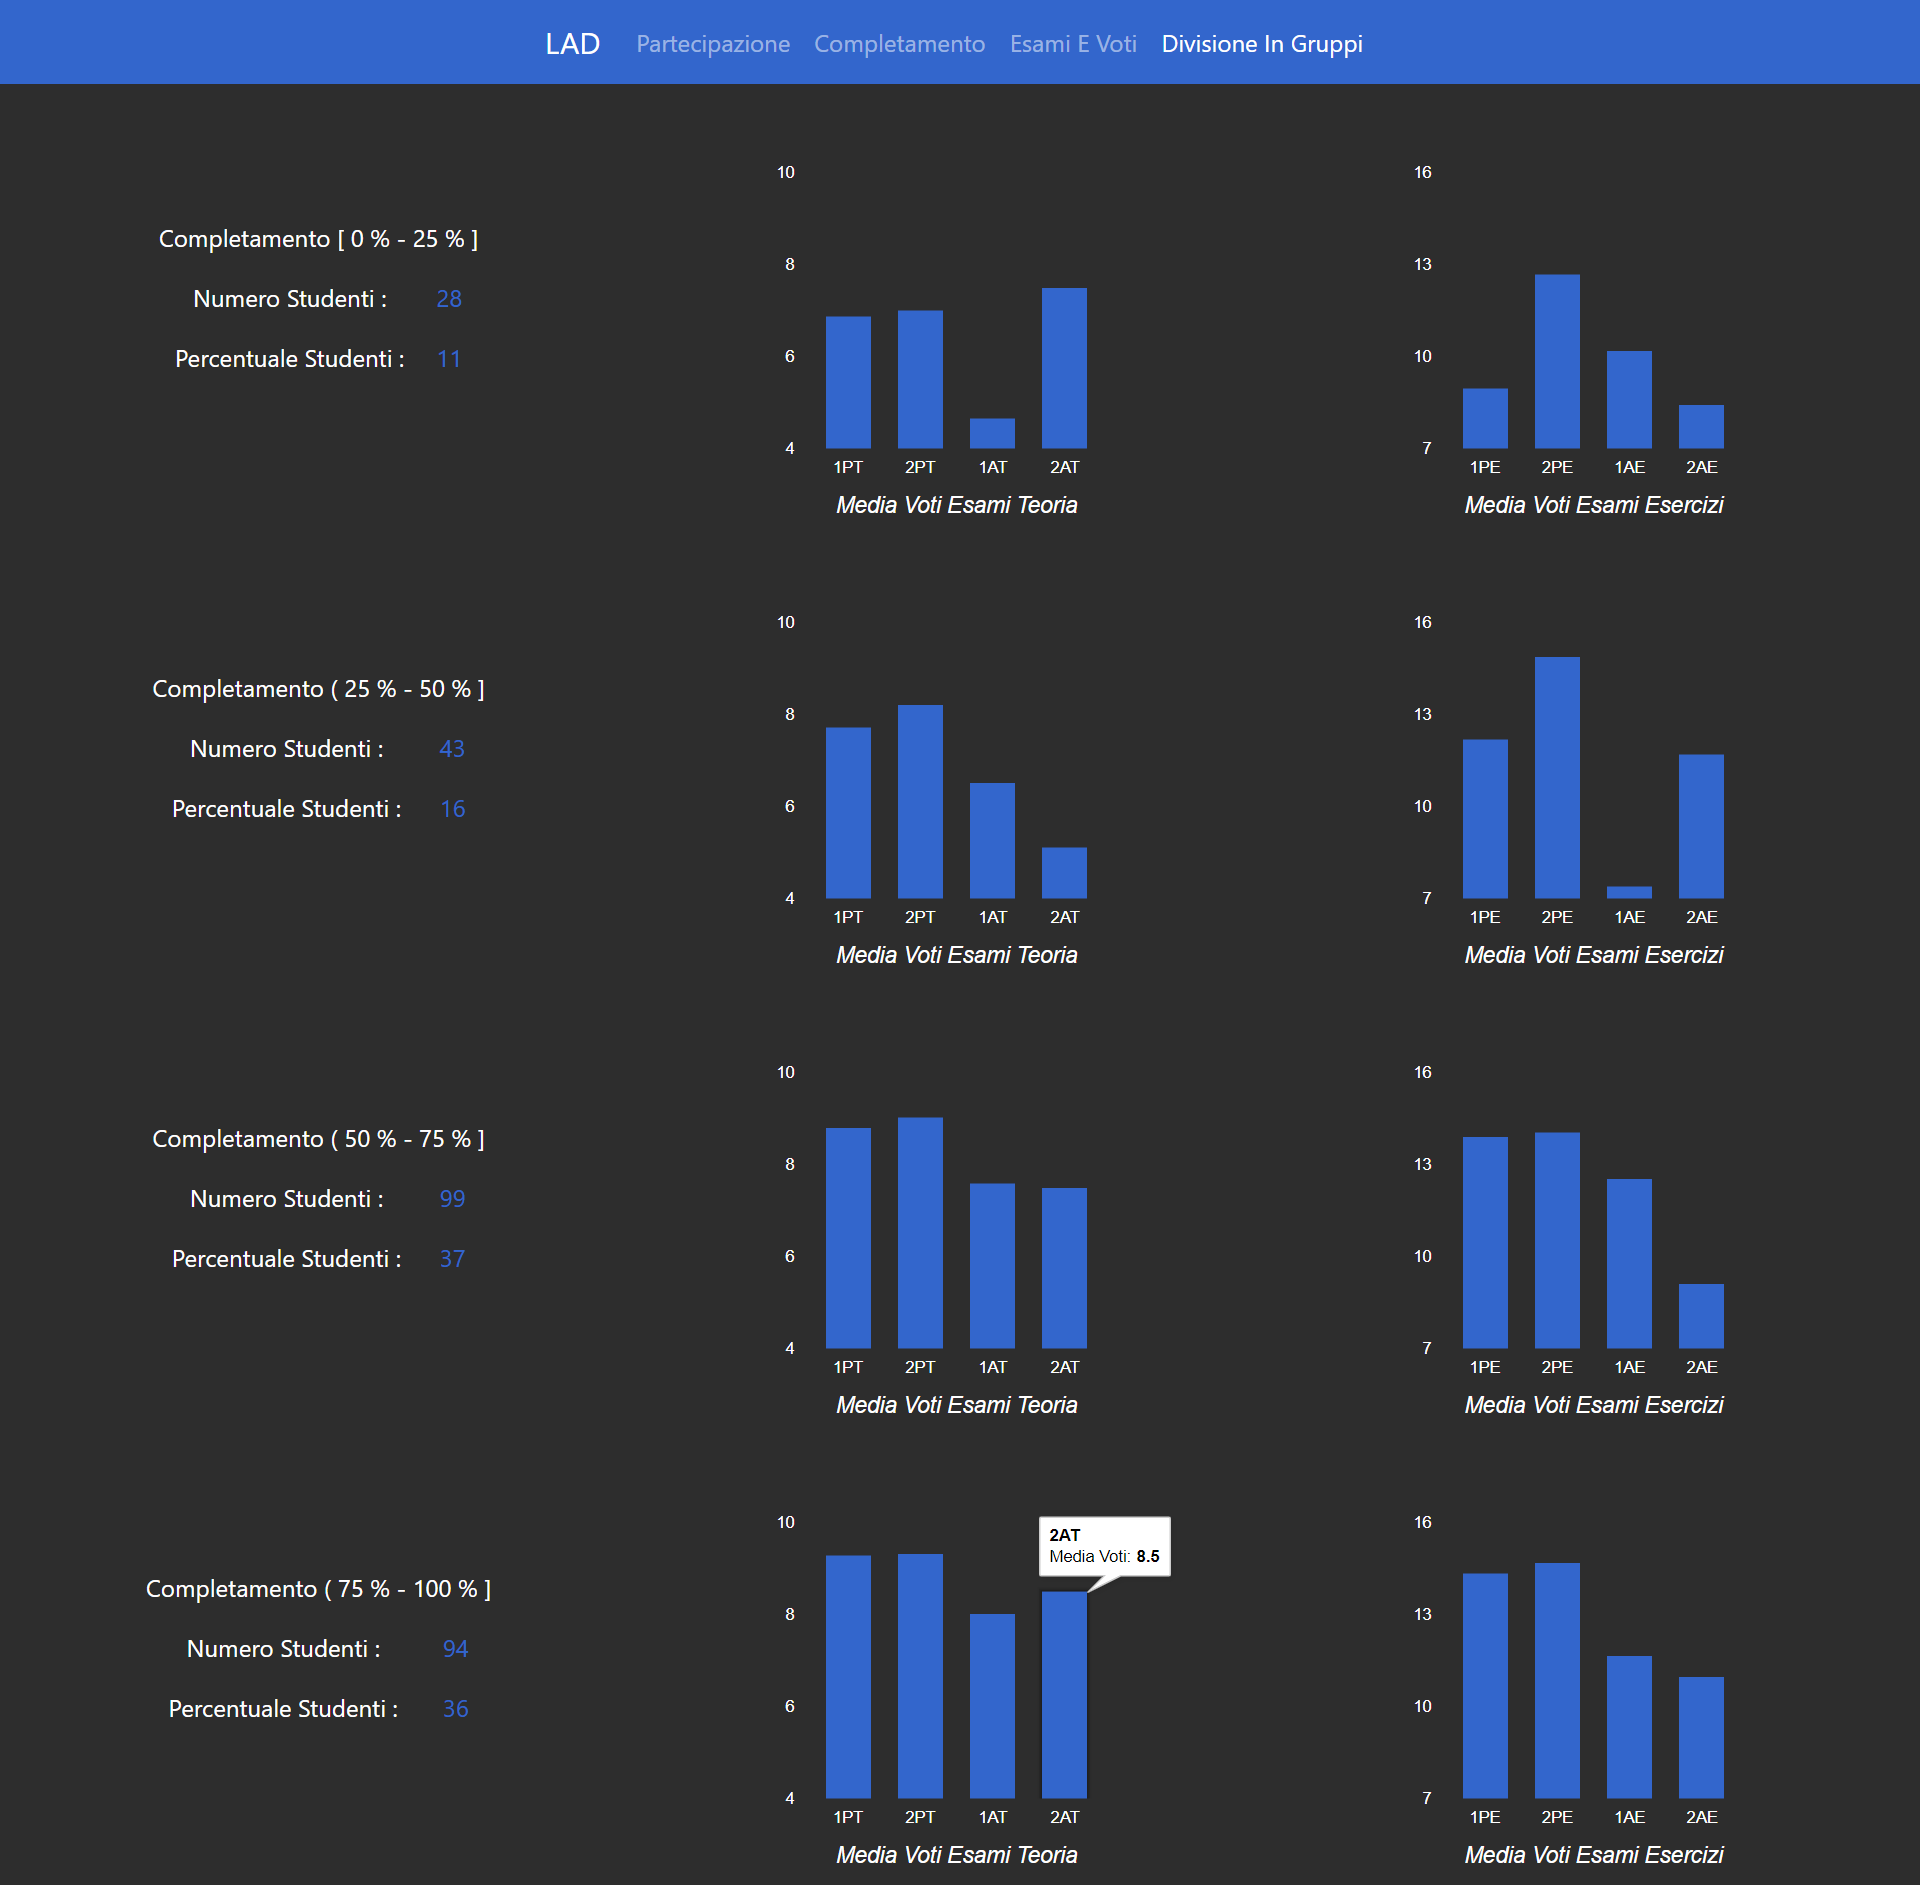
\includegraphics[width=160mm,height= 210mm]{../Immagini/8}
\end{figure}

